%\newpage
%=============================--X--=============================%
\renewcommand{\thefigure}{C\arabic{figure}}
\renewcommand{\thetable}{C\arabic{table}}
\setcounter{figure}{0}
\section{Conclusões}
\label{sec:conclusao}
\begin{figure}[ht] 
    \begin{subfigure}[b]{0.5\linewidth}
        \centering
        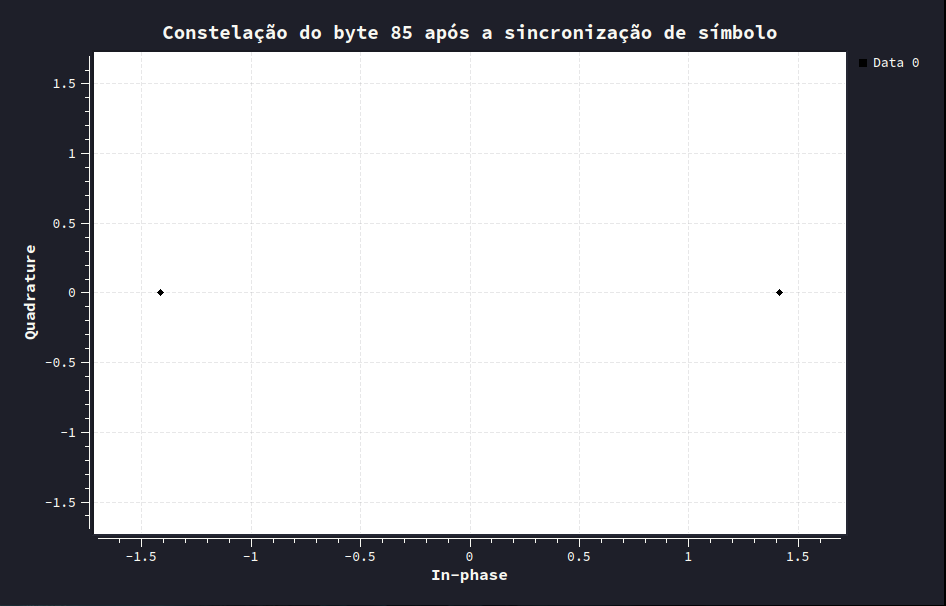
\includegraphics[width=0.8\linewidth]{img/conclusao/const-byte85-bpsk.png}
        \caption{BPSK sem \textit{noise voltage}.} 
        \label{fig:a} 
        \vspace{1ex}
    \end{subfigure}%% 
    \begin{subfigure}[b]{0.5\linewidth}
        \centering
        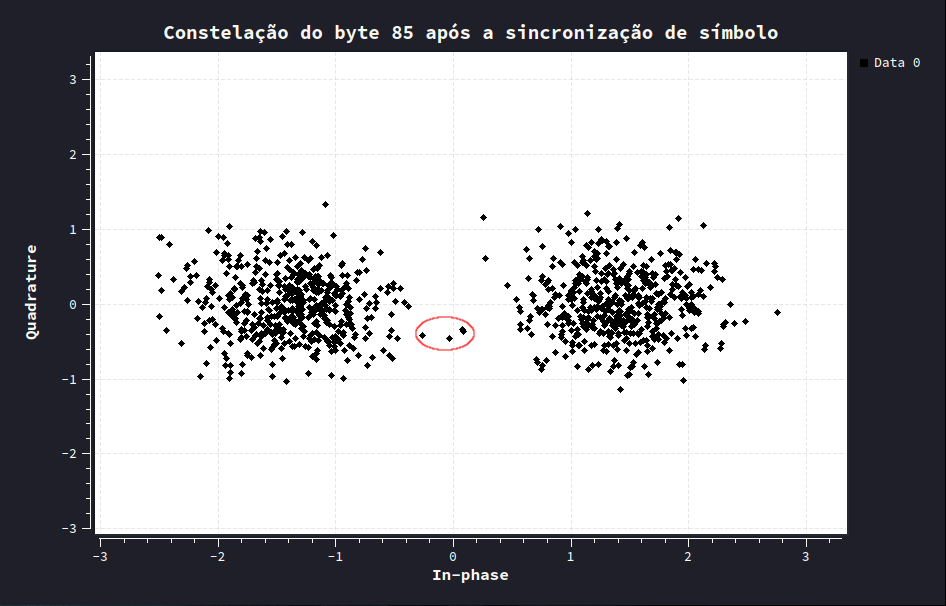
\includegraphics[width=0.8\linewidth]{img/conclusao/const-byte85-bpsk-noisy.png} 
        \caption{BPSK com 0.5 V de \textit{noise voltage}.} 
        \label{fig:b} 
        \vspace{1ex}
    \end{subfigure} 
    \begin{subfigure}[b]{0.5\linewidth}
        \centering
        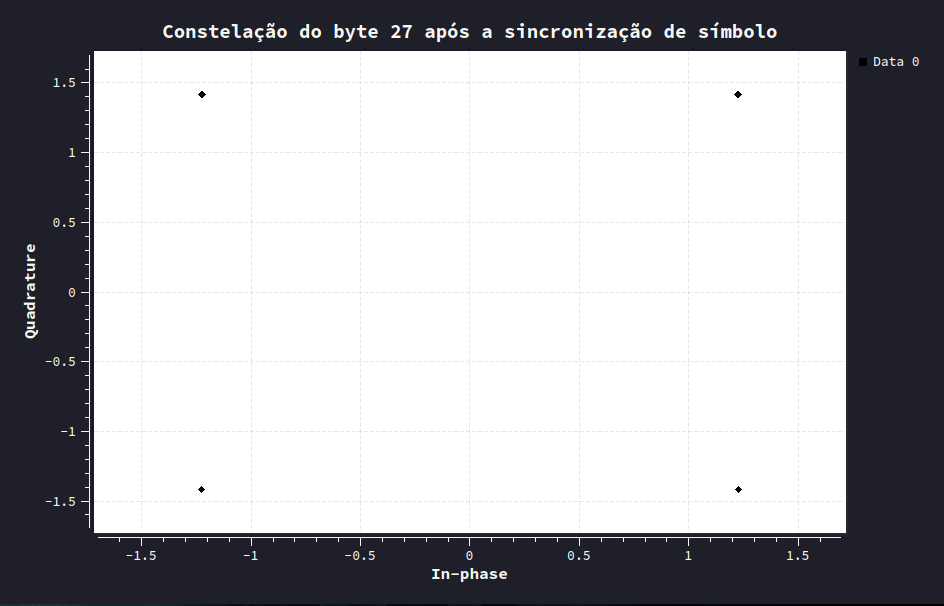
\includegraphics[width=0.8\linewidth]{img/conclusao/const-byte27-qpsk.png}
        \caption{QPSK sem \textit{noise voltage}.} 
        \label{fig:c} 
        %%\vspace{4ex}
    \end{subfigure}%% 
    \begin{subfigure}[b]{0.5\linewidth}
        \centering
        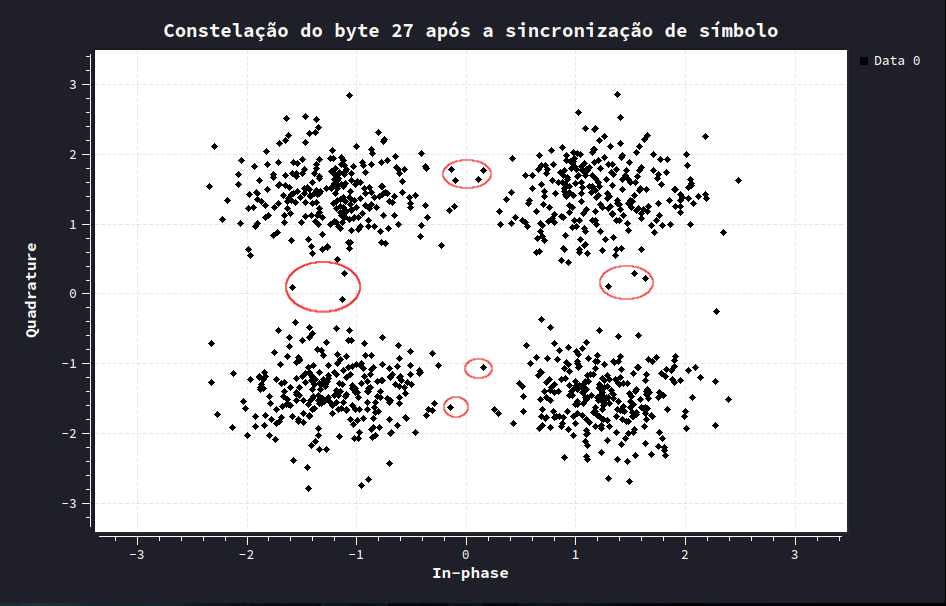
\includegraphics[width=0.8\linewidth]{img/conclusao/const-byte27-qpsk-noisy.png} 
        \caption{QPSK com 0.5 V de \textit{noise voltage}.} 
        \label{fig:d} 
        %%\vspace{4ex}
    \end{subfigure} 
    \caption{Constelações com e sem presença de AWGN.}
    \label{fig:multiplas}
\end{figure}

É conveniente aliar a discussão dos dados obtidos com a visualização dos diagramas de constelação perante a influência de ruído. Na \hyperref[fig:multiplas]{Fig. C1} encontram-se explicitadas a \textcolor{red}{vermelho} amostras situadas numa região de indecisão face à presença de AWGN (ambiguidade na decisão entre \textit{bit} `0' ou `1', vide a \hyperref[subsubsec:stream-to-bit]{secção 3.2}).

Trivialmente se correlacionam os dados adquiridos (ver \hyperref[tab:bpsk]{Tab. E1} e \hyperref[tab:qpsk]{Tab. E2}, e respetivas análises gráfica) com este fenómeno---é aparente que com o aumento do AWGN, há uma tendência (geral) esmagadora, quase obrigatória, para o aumento do número de \textit{bits} nestas zonas litigiosas (graças à dificuldade na deteção do pulso no seio do ruído, como apresentado anteriormente $\xrightarrow[]{}$ redução da relação sinal-ruído).

\begin{figure}[H]
    \centering
    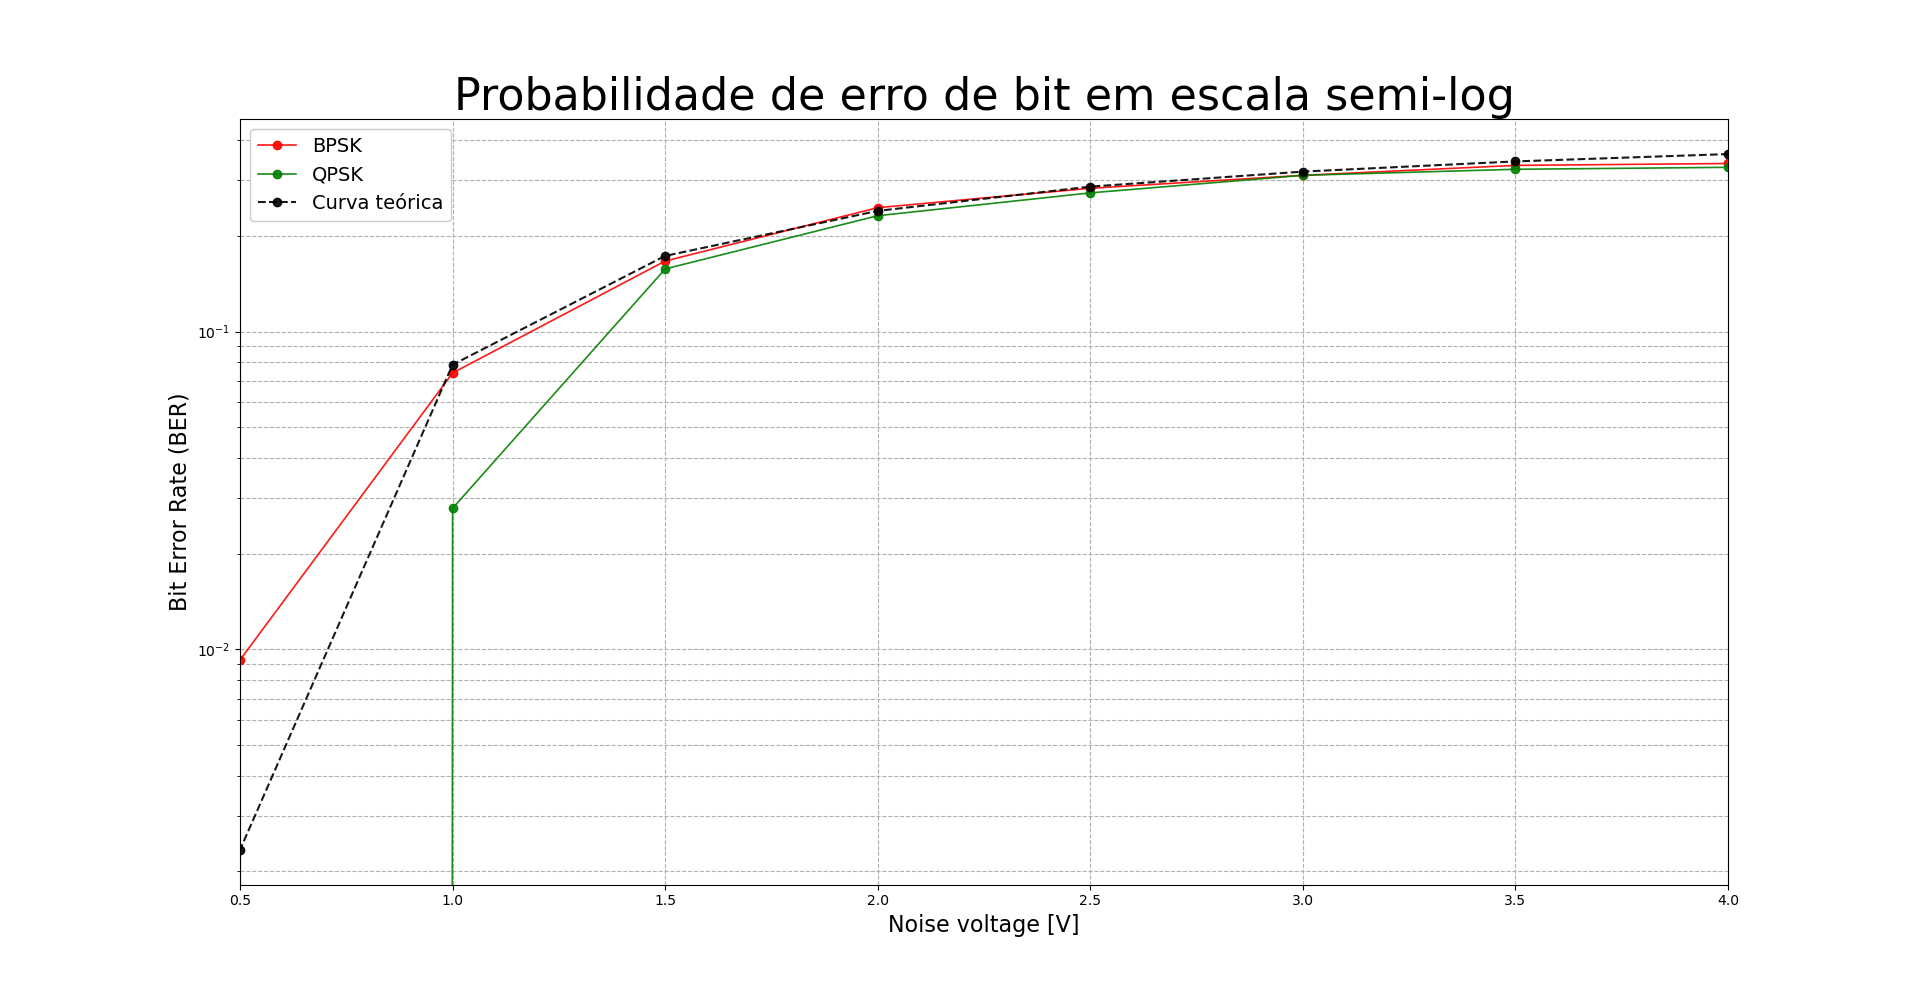
\includegraphics[width=1\linewidth]{img/conclusao/BER_plot.png}
    \caption{Curvas de probabilidade de erro de \textit{bit} (BER) em escala semi-logarítmica: \textcolor{red}{BPSK}, \textcolor{green}{QPSK} e \textcolor{black}{teórica}\protect\footnotemark[12].}
    \label{fig:BERcurves}
\end{figure}

\footnotetext[12]{As curvas \textcolor{red}{BPSK} e \textcolor{green}{QPSK} são computadas mediante a menor taxa de erro de \textit{bit} observada nas tabelas apresentadas para cada patamar de ruído; e a devida curva teórica é obtida com base na expressão supramencionada na \hyperref[subsubsec:prob-erro]{secção 4.1}, aplicada sobre o \textit{range} discreto de \textit{noise voltages} para $\sqrt{E_b} = \sqrt{2}$ (distância à origem visualizada experimentalmente em ambiente \textit{GNU Radio}).}

Não obstante, a sobreposição das curvas apresentadas na \hyperref[fig:BERcurves]{Fig. C2} verifica a similaridade (esperada e bastante proeminente por análise direta das tabelas expostas) entre as probabilidades de erro de \textit{bit} e ratifica o conteúdo teórico---sucintamente condensado na seguinte citação:
\begin{quote}
    "The biggest and primary advantage of QPSK over BPSK is spectral efficiency: for the same BER performance and data rate we can use half the bandwidth! This is also intuitively explained that we are sending two BPSK signals independently in the same bandwidth."\cite{jstraughjstraugh}
\end{quote}